\documentclass[a4paper,10pt]{article}

% ---------------------------
% Pacchetti di base
% ---------------------------
\usepackage[utf8]{inputenc}
\usepackage[T1]{fontenc}
\usepackage[italian]{babel}
\usepackage{geometry}
\geometry{margin=2cm}

% ---------------------------
% Grafica e matematica
% ---------------------------
\usepackage{graphicx}
\usepackage{amsmath, amssymb}
\usepackage{float} % Per il posizionamento preciso delle figure

% ---------------------------
% Riferimenti e link
% ---------------------------
\usepackage{hyperref}
\usepackage{bookmark}

% ---------------------------
% Header e footer
% ---------------------------
\usepackage{fancyhdr}
\fancyhf{}
\rhead{Relazione Alessandro Bertolazzi}
\cfoot{\thepage}
\pagestyle{fancy}
\setlength{\headheight}{14.5pt}

% ---------------------------
% Caption senza "Figura X:"
% ---------------------------
\usepackage[labelformat=empty]{caption}

% ---------------------------
% Listings e codice JSON e C++
% ---------------------------
\usepackage{bera}
\usepackage{listings}
\usepackage{xcolor}

% Colori di base
\definecolor{background}{HTML}{EEEEEE}
\definecolor{bluekeywords}{rgb}{0.13,0.13,1}
\definecolor{greencomments}{rgb}{0,0.5,0}
\definecolor{redstrings}{rgb}{0.9,0,0}

% Stile per C++
\lstdefinestyle{cppstyle}{
    basicstyle=\ttfamily\small,
    numbers=left,
    numberstyle=\scriptsize,
    stepnumber=1,
    numbersep=8pt,
    showstringspaces=false,
    breaklines=true,
    frame=lines,
    backgroundcolor=\color{background},
    keywordstyle=\color{bluekeywords}\bfseries,
    commentstyle=\color{greencomments},
    stringstyle=\color{redstrings},
    identifierstyle=\color{black},
    literate=
    {à}{{\`a}}1 {è}{{\`e}}1 {é}{{\'e}}1 {ì}{{\`i}}1 {ò}{{\`o}}1 {ù}{{\`u}}1
}

\lstdefinelanguage{cpp}{
    style=cppstyle,
    keywords={class, public, private, protected, virtual, override, const, auto, return, void, bool, int, double, float, char, string, vector, pair, include, using, namespace, std, constexpr, noexcept, true, false, nullptr},
    morecomment=[l]{//},
    morecomment=[s]{/*}{*/},
    morestring=[b]",
}

% Stile per JSON
\lstdefinestyle{jsonstyle}{
    basicstyle=\ttfamily\small,
    numbers=left,
    numberstyle=\scriptsize,
    stepnumber=1,
    numbersep=8pt,
    showstringspaces=false,
    breaklines=true,
    frame=lines,
    backgroundcolor=\color{background},
    literate=
     *{0}{{{\color{magenta!60!black}0}}}{1}
      {1}{{{\color{magenta!60!black}1}}}{1}
      {2}{{{\color{magenta!60!black}2}}}{1}
      {3}{{{\color{magenta!60!black}3}}}{1}
      {4}{{{\color{magenta!60!black}4}}}{1}
      {5}{{{\color{magenta!60!black}5}}}{1}
      {6}{{{\color{magenta!60!black}6}}}{1}
      {7}{{{\color{magenta!60!black}7}}}{1}
      {8}{{{\color{magenta!60!black}8}}}{1}
      {9}{{{\color{magenta!60!black}9}}}{1}
      {:}{{{\color{red!60!black}{:}}}}{1}
      {,}{{{\color{red!60!black}{,}}}}{1}
      {\{}{{{\color{blue!60!black}{\{}}}}{1}
      {\}}{{{\color{blue!60!black}{\}}}}}{1}
      {[}{{{\color{blue!60!black}{[}}}}{1}
      {]}{{{\color{blue!60!black}{]}}}}{1}
      {"}{{{\color{red!60!black}"}}}{1},
}

% ---------------------------
% Tabelle avanzate
% ---------------------------
\usepackage{tabularx}
\renewcommand{\arraystretch}{1.3} % Più spazio tra righe

% ---------------------------
% Titolo
% ---------------------------
\title{Relazione progetto Programmazione ad Oggetti}
\author{Alessandro Bertolazzi \\ 1227274}
\date{}

\begin{document}

\maketitle

\begin{abstract}
\noindent Relazione del progetto "Biblioteca Virtuale" per il corso "Programmazione ad Oggetti". Un'applicazione scritta in C++ con framework Qt che permette la gestione di una biblioteca personale, implementando design pattern avanzati e un'architettura modulare scalabile.
\end{abstract}

\section{Introduzione}
Bibliotheca procurator dal latino "direttore della biblioteca", il nome che ho deciso di dare all'applicazione. Il progetto proponeva di creare un'applicazione che permettesse la gestione di una biblioteca. L'applicazione che ho sviluppato non riguarda l'organizzazione di una biblioteca pubblica, bensì l'organizzazione di una biblioteca privata in modo da poter strutturare e catalogare libri, film, CD, manga, anime e serie TV per un privato con collezioni ampie. Mi sono dedicato a questo obiettivo poiché, oltre a poter avere un'utilità per me stesso, ho notato che non si trovano prodotti simili online e, se si trovano, si tratta di applicazioni datate, a pagamento o non più mantenute.

\section{Struttura del Progetto}
\subsection{Logic}
Nella cartella \texttt{Logic} si trova tutta la parte logica dell'applicazione. Ho implementato 6 classi concrete: \texttt{Anime}, \texttt{SerieTv}, \texttt{Film}, \texttt{Cd}, \texttt{Manga} e \texttt{Libro}. Come classi astratte ho utilizzato \texttt{Media} come superclasse e due classi intermedie \texttt{Series} e \texttt{Cartaceo} per raggruppare funzionalità comuni. Ho inoltre implementato il pattern Visitor tramite \texttt{MediaVisitor} per gestire operazioni polimorfiche sui diversi tipi di media.

\begin{figure}[ht!]
    \centering
    
\includegraphics[width=0.6\textwidth]{img/DisegnoSchemaLogico.png}
    \caption{Struttura logica dell'applicazione}
\end{figure}

\newpage

\subsection{UI}
Per l'interfaccia grafica ho adottato un'architettura modulare dove \texttt{mainWindow} coordina diversi widget specializzati:

\begin{itemize}
    \item \texttt{topMenuWidget}: gestisce la barra superiore con pulsanti iconografici per le operazioni principali (carica, salva, crea, toggle tema)
    \item \texttt{rightLayoutWidget}: si occupa della visualizzazione dinamica dei media utilizzando il pattern Visitor per creare widget specifici per ogni tipo
    \item \texttt{createItemWidget}: finestra modulare per creazione e modifica che utilizza form generati dinamicamente tramite \texttt{FormWidgetVisitor}
    \item \texttt{mediaWidgetVisitor}: implementa il pattern Visitor per creare rappresentazioni UI specifiche per ogni tipo di media
    \item \texttt{formWidgetVisitor}: genera automaticamente form di inserimento/modifica basati sul tipo di media selezionato
\end{itemize}

\subsection{Services}
Ho implementato un'architettura a servizi:

\begin{itemize}
    \item \texttt{JsonService}: gestisce la persistenza dei dati utilizzando un pattern Factory per la creazione dinamica di oggetti Media dal JSON
    \item \texttt{MediaService}: service layer principale che incapsula tutta la business logic per la gestione dei media, inclusi validazione, operazioni CRUD e filtering
    \item \texttt{UIService}: si occupa della formattazione dei dati per la visualizzazione e della gestione delle immagini con placeholder automatici
    \item \texttt{StyleUtils}: sistema centralizzato di gestione degli stili con supporto per temi chiaro/scuro e palette di colori coerenti
    \item \texttt{JsonTypeVisitor}: visitor specializzato per determinare il tipo di media durante la serializzazione
\end{itemize}

\section{Design Pattern Implementati}

\subsection{Visitor Pattern}
Il Visitor pattern è stato implementato in diversi contesti per separare gli algoritmi dalle strutture dati:

\begin{lstlisting}[language=cpp, style=cppstyle]
class MediaVisitor {
public:
    virtual ~MediaVisitor() = default;
    virtual void visit(Film* film) = 0;
    virtual void visit(SerieTv* serieTv) = 0;
    virtual void visit(Anime* anime) = 0;
    virtual void visit(Libro* libro) = 0;
    virtual void visit(Manga* manga) = 0;
    virtual void visit(Cd* cd) = 0;
};

// Utilizzo
media->accept(widgetVisitor);
QWidget* specificWidget = widgetVisitor->getResultWidget();
\end{lstlisting}

Ho utilizzato questo pattern per:
\begin{itemize}
    \item Creazione di widget UI specifici (\texttt{MediaWidgetVisitor})
    \item Generazione di form dinamici (\texttt{FormWidgetVisitor})  
    \item Determinazione del tipo per serializzazione (\texttt{JsonTypeVisitor})
\end{itemize}

\subsection{Factory Method Pattern}
Implementato per la creazione dinamica di oggetti Media dal JSON senza conoscere il tipo specifico a compile-time:

\begin{lstlisting}[language=cpp, style=cppstyle]
void JsonService::initializeFactories() {
    mediaFactories["Film"] = [](const QJsonObject& json) -> std::unique_ptr<Media> {
        std::string titolo = json["titolo"].toString().toStdString();
        int anno = json["anno"].toInt();
        std::string immagine = json["immagine"].toString().toStdString();
        
        auto film = std::make_unique<Film>(titolo, anno, immagine, "", "", 0);
        film->fromJsonSpecific(json);
        return film;
    };
    
    mediaFactories["Serie Tv"] = [](const QJsonObject& json) -> std::unique_ptr<Media> {
        // Factory per Serie TV...
    };
}
\end{lstlisting}

\subsection{Template Method Pattern}
Utilizzato per la validazione unificata dei form con algoritmi personalizzabili:

\begin{lstlisting}[language=cpp, style=cppstyle]
template<typename Validator>
bool MediaService::validateFieldAtIndex(const QList<QLineEdit*>& fields, int index, 
                                       const QString& fieldName, QWidget* parent, 
                                       Validator validator) const {
    if (index >= fields.size()) return false;
    return validator(fields[index], fieldName, parent);
}

auto validateFields = [this, &fields, parent](
    const QVector<QPair<int, QString>>& fieldConfigs, 
    auto validator) -> bool {
    for (const auto& field : fieldConfigs) {
        if (!validateFieldAtIndex(fields, field.first, field.second, parent, validator)) {
            return false;
        }
    }
    return true;
};
\end{lstlisting}

\section{Persistenza dei Dati}
Ho implementato un sistema di persistenza basato su JSON. Implementando \textbf{Factory Pattern} per la creazione dinamica di oggetti dal JSON, \textbf{Template Method} per la serializzazione/deserializzazione specifica per tipo, \textbf{Visitor Pattern} per determinare il tipo durante la serializzazione. Ogni classe concreta implementa metodi virtuali per la gestione specifica dei propri dati:

\begin{lstlisting}[language=cpp, style=cppstyle]
// Metodi virtuali per serializzazione
virtual QJsonObject toJsonSpecific() const = 0;
virtual void fromJsonSpecific(const QJsonObject& json) = 0;

QJsonObject SerieTv::toJsonSpecific() const {               // Implementazione in SerieTv
    auto json = getSeriesBaseJson(); // Eredita da Series
    json["type"] = "Serie Tv";
    json["ideatore"] = QString::fromStdString(ideatore);
    json["casaProduttrice"] = QString::fromStdString(casaProduttrice);
    return json;
}
\end{lstlisting}
Il file JSON é cosi strutturato:

\begin{lstlisting}[style=jsonstyle]
"media": [    {
        "anno": 1986,
        "disegnatore": "Akira Toriyama",
        "durataMediaEp": 24,
        "immagine": "../resources/img/dragonball.jpg",
        "inCorso": false,
        "numEpisodi": 153,
        "numStagioni": 5,
        "studioAnimazione": "Toei Animation",
        "titolo": "Dragon Ball",
        "type": "Anime"
    }]
\end{lstlisting}

\section{Polimorfismo e Architettura Modulare}

\subsection{Serializzazione Polimorfica}
Ho eliminato l'uso di dynamic\_cast sostituendolo con metodi virtuali per una gestione più pulita e sicura:

\begin{lstlisting}[language=cpp, style=cppstyle]
virtual QJsonObject toJsonSpecific() const = 0;
virtual void fromJsonSpecific(const QJsonObject& json) = 0;
virtual Media* clone() const = 0;
virtual bool matchesCategory(const string& category) const = 0;
\end{lstlisting}

\subsection{Gestione Memory-Safe}
Utilizzo di smart pointer e RAII (Resource Acquisition Is Initialization) per una gestione automatica della memoria:

\begin{lstlisting}[language=cpp, style=cppstyle]
std::function<std::unique_ptr<Media>(const QJsonObject&)> mediaFactories;

Media* Anime::clone() const {       // Clone pattern per duplicazione
    return new Anime(getTitolo(), getAnno(), getImmagine(), 
                    getNumEpisodi(), getNumStagioni(), getDurataMediaEp(), 
                    getInCorso(), disegnatore, studioAnimazione);
}
\end{lstlisting}

\section{Form Dinamici e UI Generata}
Il sistema di creazione/modifica utilizza form generati automaticamente tramite il pattern Visitor:

\begin{lstlisting}[language=cpp, style=cppstyle]
const QVector<FieldConfig> FILM_FIELDS = {       // Configurazioni statiche per ogni tipo di media
    {"Titolo", "Inserisci titolo"},
    {"Immagine", "Inserisci percorso immagine", FieldType::IMAGE},
    {"Anno", "Inserisci anno", FieldType::INTEGER},
    {"Regista", "Inserisci regista"},
    {"Attore Protagonista", "Inserisci attore protagonista"},
    {"Durata (min)", "Inserisci durata in minuti", FieldType::POSITIVE_INTEGER}
};

template<typename MediaType>    // Generazione automatica del form
void FormWidgetVisitor::visitGeneric(MediaType* media, const QVector<FieldConfig>& fieldConfigs) {
    QStringList values;
    if (media) {
        values = extractValues(media);
    }
    resultWidget = createStandardForm(fieldConfigs, values);
}
\end{lstlisting}

\newpage

\section{Interfaccia Grafica}

\begin{figure}[ht!]
    \centering
    \begin{minipage}{0.4\textwidth}
        
\includegraphics[width=\linewidth]{img/TopButton.png}
    \end{minipage}\hfill
    \begin{minipage}{0.55\textwidth}
        \small
        Barra superiore con sistema iconografico:
        \begin{itemize}
            \item Carica biblioteca esistente
            \item Crea nuova biblioteca con auto-save della cache
            \item Chiudi biblioteca corrente
            \item Crea nuovo elemento media
            \item Toggle tema chiaro/scuro dinamico
        \end{itemize}
    \end{minipage}
\end{figure}

\begin{figure}[ht!]
    \centering
    \begin{minipage}{0.4\textwidth}
        
\includegraphics[width=\linewidth]{img/LeftMenu.png}
    \end{minipage}\hfill
    \begin{minipage}{0.55\textwidth}
        \small
        Nel leftMenu viene creata la barra di ricerca che, ad ogni cambiamento (ogni volta che viene digitato un carattere), cerca l’elemento nella biblioteca. La ricerca è  "case insensitive" e funziona anche con ricerca parziale. Sotto sono presenti i media categorizzati per tipologia.
    \end{minipage}
\end{figure}

\begin{figure}[ht!]
    \centering
    \begin{minipage}{0.4\textwidth}
        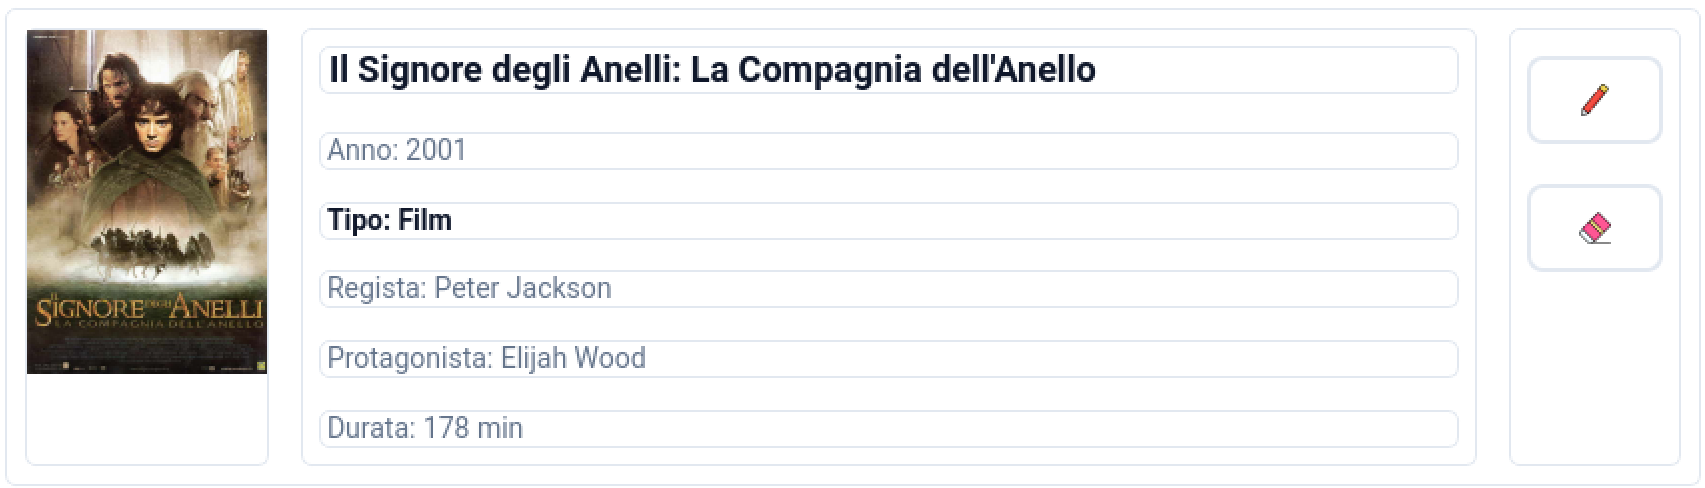
\includegraphics[width=\linewidth]{img/MediaItem.png}
    \end{minipage}\hfill
    \begin{minipage}{0.55\textwidth}
        \small
        Ogni elemento media utilizza il pattern Visitor per generare layout specifici con:
        \begin{itemize}
            \item Caricamento delle immagini
            \item Bottoni di azione per la modifica e la cancellazione
            \item Layout responsive che si adatta al contenuto
            \item Dettagli specifici per ogni tipo di media
        \end{itemize}
    \end{minipage}
\end{figure}

\section{Ricerca e Filtering}
Ho implementato un sistema di ricerca case-insensitive con filtering per categorie:

\begin{lstlisting}[language=cpp, style=cppstyle]
bool Media::matchesSearch(const string& searchText) const {
    if (searchText.empty()) return true;
    
    string lowerTitle = titolo;
    string lowerSearch = searchText;
    
    // Conversione case-insensitive
    std::transform(lowerTitle.begin(), lowerTitle.end(), lowerTitle.begin(), ::tolower);
    std::transform(lowerSearch.begin(), lowerSearch.end(), lowerSearch.begin(), ::tolower);
    
    return lowerTitle.find(lowerSearch) != string::npos;
}

// Filtering combinato categoria + ricerca
QVector<Media*> MediaService::filterMedia(const QString& category, const QString& searchText) const {
    QVector<Media*> filtered;
    std::string categoryStd = category.toStdString();
    std::string searchStd = searchText.toStdString();
    
    for (Media* media : mediaCollection) {
        if (media->matchesCategory(categoryStd) && media->matchesSearch(searchStd)) {
            filtered.append(media);
        }
    }
    return filtered;
}
\end{lstlisting}

\section{Rendiconto delle Tempistiche}
Lo sviluppo del progetto ha richiesto circa 80 ore di lavoro, distribuite come segue:

\begin{table}[h!]
\centering
\begin{tabularx}{\textwidth}{p{4cm} p{2cm} p{2cm} X}
\hline
\textbf{Jobs} & \textbf{Scheduled hours} & \textbf{Actual hours} & \textbf{Notes} \\
\hline
Modellazione diagramma UML          & 1  & 2  & Tempo aggiuntivo per progettazione pattern \\
Implementazione modello Logico      & 5  & 6  & Aggiunta pattern Visitor e metodi virtuali \\
Implementazione Design Pattern      & 8  & 12 & Visitor, Factory, Template Method \\
Implementazione Interfaccia grafica & 15 & 20 & Sistema di temi e widget modulari \\
Implementazione parte Service       & 15 & 18 & Architettura a servizi e validazione \\
Sistema di Validazione              & 5  & 8  & Validazione robusta con template \\
Affinamento Progetto                & 5  & 8  & UI/UX improvements e ottimizzazioni \\
Debug e Testing                     & 5  & 6  & Testing approfondito e correzioni \\
\hline
\end{tabularx}
\end{table}

\section{Possibili Miglioramenti}
\begin{itemize}
    \item Implementare una ricerca online automatica delle copertine dei media
    \item Per Serie TV, Anime e Manga, permettere all'utente di specificare quali volumi/episodi possiede effettivamente
    \item Migliorare il sistema di scaling e ridimensionamento delle immagini
    \item Aggiungere supporto per database relazionali oltre al JSON
    \item Implementare sistema di backup automatico e cronologia delle modifiche
    \item Aggiungere statistiche avanzate sulla collezione con grafici
    \item Supportare collezioni multiple e condivisione tra utenti
    \item Implementare sistema di importazione da cataloghi online (IMDb, MyAnimeList, etc.)
\end{itemize}

\section{Conclusioni}
Il progetto Bibliotheca Procurator rappresenta un'applicazione per la gestione di biblioteche personali che implementa diversi design pattern avanzati e un'architettura modulare scalabile. L'uso del pattern Visitor per la generazione dinamica dell'UI, del Factory pattern per la persistenza dei dati, e del Template Method per la validazione, combinati con un sistema di servizi, rendono l'applicazione facilmente estensibile e manutenibile.

\section{Terminologie Utilizzate}
\begin{itemize}
    \item \textbf{Factory Method Pattern}: Pattern creazionale implementato tramite lambda functions in \texttt{JsonService} per creare istanze specifiche di Media dal JSON senza conoscere il tipo a compile-time.
    \item \textbf{Visitor Pattern}: Pattern comportamentale utilizzato per separare algoritmi dalle strutture dati, implementato per generazione UI (\texttt{MediaWidgetVisitor}), form dinamici (\texttt{FormWidgetVisitor}) e serializzazione (\texttt{JsonTypeVisitor}).
    \item \textbf{Template Method Pattern}: Pattern utilizzato per definire algoritmi di validazione con parti personalizzabili, implementato tramite template functions in \texttt{MediaService}.
    \item \textbf{Service Layer Architecture}: Architettura che separa la business logic in servizi specializzati (\texttt{MediaService}, \texttt{JsonService}, \texttt{UIService}, \texttt{StyleUtils}).
    \item \textbf{SOLID Principles}: Principi di design object-oriented applicati per garantire codice mantenibile e estensibile.
    \item \textbf{Media}: Termine generico per indicare qualsiasi elemento della collezione (Film, Libro, CD, Serie TV, Anime, Manga).
    \item \textbf{Smart Pointers}: Utilizzo di \texttt{std::unique\_ptr} per gestione automatica della memoria e ownership chiara.
    \item \textbf{RAII (Resource Acquisition Is Initialization)}: Tecnica di gestione delle risorse che lega il ciclo di vita delle risorse a quello degli oggetti.
\end{itemize}

\end{document}